\documentclass{standalone}
\usepackage{tikz}
\usetikzlibrary{shapes}
\begin{document}
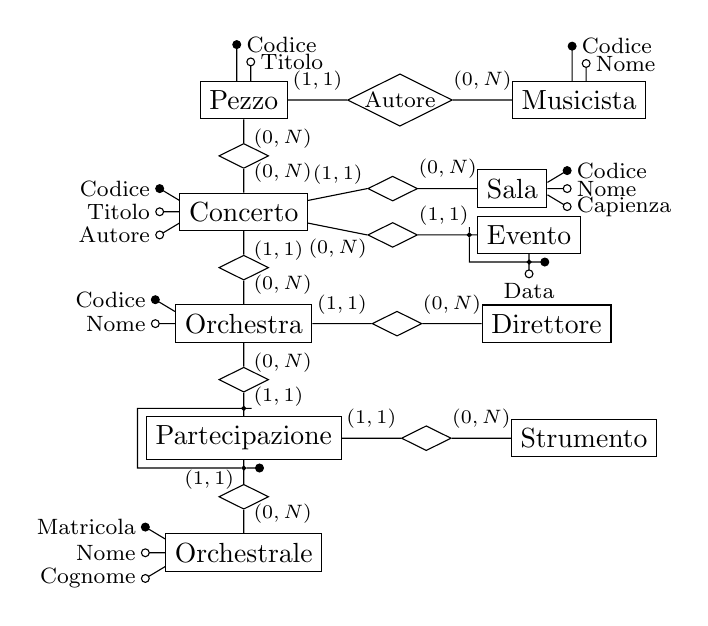
\begin{tikzpicture}
    \draw

    %%* Attributi:
    %%  node[draw, circle, inner sep=1pt,anchor=180, fill=black]{}node[right]{\footnotesize A}
    %%? Distanza orizzontale: E -(0.25,0.x)- A
    %%? Distanza verticale: E -(0,x * 0.22)- A

    %%* Cardinalità:
    %%  node[below right]{\scriptsize $(0,N)$}
    %%  node[above right]{\scriptsize $(0,N)$}
    %%  node[midway, above]{\scriptsize $(0,N)$}

    %%* Relazione:
    %% node[draw, diamond, shape aspect=2, inner sep=3pt, anchor=90](r1){}
    %% node[draw, diamond, shape aspect=2, inner sep=0.2pt, anchor=180](r2){R2}

    %%* Entità:
    %% node[draw, rectangle, anchor=90](e1){}
    %%? Distanza verticale: E -(0.3)- R -(0.3) E
    %%? Distanza orizzontale: E -(0.75)- R -(0.75)- E


    %%* Pezzo
    (0,0)node[draw, rectangle, anchor=90](pezzo){Pezzo}
    (pezzo.110)--++(0,0.46)node[draw, circle, inner sep=1pt, fill=black]{}node[right]{\footnotesize Codice}
    (pezzo.70)--++(0,0.24)node[draw, circle, inner sep=1pt, fill=white]{}node[right]{\footnotesize Titolo}


    %%* Musicista
    (pezzo.0)--++(0.75,0)node[midway, above]{\scriptsize $(1,1)$}node[draw, diamond, shape aspect=2, inner sep=0.2pt, anchor=180](r3){\footnotesize Autore}
    (r3.0)--++(0.75,0)   node[midway, above]{\scriptsize $(0,N)$}node[draw, rectangle, anchor=180](musicista){Musicista}
    (musicista.110)--++(0,0.44)node[draw, circle, inner sep=1pt, fill=black]{}node[right]{\footnotesize Codice}
    (musicista.70)--++(0,0.22) node[draw, circle, inner sep=1pt, fill=white]{}node[right]{\footnotesize Nome}


    %%* Concerto
    (pezzo.270)node[below right]{\scriptsize $(0,N)$}--++(0,-0.3)node[draw, diamond, shape aspect=2, inner sep=3pt, anchor=90](r1){}
    (r1.270)--++(0,-0.3)node[above right]{\scriptsize $(0,N)$}node[draw, rectangle, anchor=90](concerto){Concerto}
    (concerto.170)--++(-0.25,0.15) node[draw, circle, inner sep=1pt, fill=black]{}node[left]{\footnotesize Codice}
    (concerto.180)--++(-0.25,0)    node[draw, circle, inner sep=1pt, fill=white]{}node[left]{\footnotesize Titolo}
    (concerto.190)--++(-0.25,-0.15)node[draw, circle, inner sep=1pt, fill=white]{}node[left]{\footnotesize Autore}
    

    %%* Sala
    (concerto.10)--++(0.75,0.15)node[midway, above]{\scriptsize $(1,1)$}node[draw, diamond, shape aspect=2, inner sep=3pt, anchor=180](r8){}
    (r8.0)--++(0.75,0)node[midway, above]{\scriptsize $(0,N)$}node[draw, rectangle, anchor=180](sala){Sala}
    (sala.10)--++(0.25,0.15)  node[draw, circle, inner sep=1pt, fill=black]{}node[right]{\footnotesize Codice}
    (sala.0)--++(0.25,0)      node[draw, circle, inner sep=1pt, fill=white]{}node[right]{\footnotesize Nome}
    (sala.350)--++(0.25,-0.15)node[draw, circle, inner sep=1pt, fill=white]{}node[right]{\footnotesize Capienza}


    %%* Evento
    (concerto.350)--++(0.75,-0.15)node[midway, below]{\scriptsize $(0,N)$}node[draw, diamond, shape aspect=2, inner sep=3pt, anchor=180](r9){}
    (r9.0)--++(0.65,0)node[midway, above]{\scriptsize $(1,1)$}node[draw, circle, inner sep=0.5pt, fill=black](a){}--++(0.10,0)node[draw, rectangle, anchor=180](evento){Evento}
    (evento.270)--++(0,-0.1)node[draw, circle, inner sep=0.5pt, fill=black](b){}--++(0,-0.15)node[draw, circle, inner sep=1pt, fill=white]{}node[below]{\footnotesize Data}
    (b)++(0.2,0)node[draw, circle, inner sep=1pt, fill=black]{}-|(a)--++(0,0.1)


    %%* Orchestra
    (concerto.270)node[below right]{\scriptsize $(1,1)$}--++(0,-0.3)node[draw, diamond, shape aspect=2, inner sep=3pt, anchor=90](r2){}
    (r2.270)--++(0,-0.3)node[above right]{\scriptsize $(0,N)$}node[draw, rectangle, anchor=90](orchestra){Orchestra}
    (orchestra.170)--++(-0.25,0.15) node[draw, circle, inner sep=1pt, fill=black]{}node[left]{\footnotesize Codice}
    (orchestra.180)--++(-0.25,0)    node[draw, circle, inner sep=1pt, fill=white]{}node[left]{\footnotesize Nome}


    %%* Direttore
    (orchestra.0)--++(0.75,0)node[midway, above]{\scriptsize $(1,1)$}node[draw, diamond, shape aspect=2, inner sep=3pt, anchor=180](r4){}
    (r4.0)--++(0.75,0)node[midway, above]{\scriptsize $(0,N)$}node[draw, rectangle, anchor=180](direttore){Direttore}


    %%* Partecipazione
    (orchestra.270)node[below right]{\scriptsize $(0,N)$}--++(0,-0.3)node[draw, diamond, shape aspect=2, inner sep=3pt, anchor=90](r6){}
    (r6.270)--++(0,-0.2)node[draw, circle, inner sep=0.5pt, fill=black](a){}--++(0,-0.1)node[above right]{\scriptsize $(1,1)$}node[draw, rectangle, anchor=90](partecipazione){Partecipazione}


    %%* Strumento
    (partecipazione.0)--++(0.75,0)node[midway, above]{\scriptsize $(1,1)$}node[draw, diamond, shape aspect=2, inner sep=3pt, anchor=180](r7){}
    (r7.0)--++(0.75,0)   node[midway, above]{\scriptsize $(0,N)$}node[draw, rectangle, anchor=180](strumento){Strumento}    


    %%* Orchestrale
    (partecipazione.270)node[below left]{\scriptsize $(1,1)$}--++(0,-0.1)node[draw, circle, inner sep=0.5pt, fill=black](b){}--++(0,-0.2)node[draw, diamond, shape aspect=2, inner sep=3pt, anchor=90](r5){}
    (r5.270)--++(0,-0.3)node[above right]{\scriptsize $(0,N)$}node[draw, rectangle, anchor=90](orchestrale){Orchestrale}
    (orchestrale.170)--++(-0.25,0.15) node[draw, circle, inner sep=1pt, fill=black]{}node[left]{\footnotesize Matricola}
    (orchestrale.180)--++(-0.25,0)    node[draw, circle, inner sep=1pt, fill=white]{}node[left]{\footnotesize Nome}
    (orchestrale.190)--++(-0.25,-0.15)node[draw, circle, inner sep=1pt, fill=white]{}node[left]{\footnotesize Cognome}
    %%* Identificatore Esterno
    (a)++(0.1,0)--++(-1.45,0)|-(b)--++(0.2,0)node[draw, circle, inner sep=1pt, fill=black]{}

    ;
\end{tikzpicture}
\end{document}